\documentclass[vruler,DEV,onecolumn]{COB}

\unsetvruler

\usepackage{boites}

\begin{document}

\supertitle{Research Article}

\title{How to use the Company of Biologists (\JABBR) \LaTeX\ class}

\author[First author and Second author]{First author$^{1}$ and Second author $^{2}$}

\address{\add{1}{First author address}
\add{2}{Second author address}}

\corres{\name{First author}
\email{xxxx@xxxx.xxx.xx}}

\date{Received xx xxxx xx}

\maketitle

\begin{abstract}
This sample is a guideline for preparing technical papers
using \LaTeX. It contains the documentation for a \LaTeX\
class file that creates the correct manuscript layout for
any of the Company of Biologists journals: Development,
Journal of Cell Science, Journal of Experimental Biology,
Biology Open or Disease Models and Mechanisms. This sample
file uses a class file named \texttt{COB.cls}, which
authors should use during manuscript preparation.
\end{abstract}

\keywords{keyword entry 1, keyword entry 2, keyword entry 3}

\section{Introduction}\label{sec1}

This latex class file is available for authors to prepare
their manuscript for submission to any of our journals. It is assumed that
authors are familiar with either plain \TeX, \LaTeX,\
\AmS-\TeX\ or a standard latex set-up and therefore only the
essential points are described in this document. For more
details, please go through the \textit{\LaTeX\ User's Guide} or
\textit{The not so short introduction to \LaTeXe} (which is available online).
The \verb|COB.cls| file is similar to the \texttt{article.cls} of
\LaTeX, with only a few additional changes in the preamble.

\section{Installation}
The \texttt{COB.cls} has to be copied into a directory
where tex looks for input files. The other files should be kept for
reference during the preparation of your
manuscript. Please use pre-defined commands
for title, authors, address, abstract, keywords, body etc. as shown in Box 1.

\section{How to start using COB.cls}

Before you type anything that actually appears in the paper
you need to include a \verb|\documentclass{COB}|
command at the very beginning and then, the two commands
that have to be part of any latex document,
\verb|\begin{document}| at the start and the
\verb|\end{document}| at the end of your paper.

Please use the respective option in the
\verb+\documentclass+ command to get the
appropriate journal name in the header.

\vskip1pc

{\begin{tabular}{ll}
\textit{Development} & \verb+\documentclass+\textcolor{red}{\tt[DEV]}\verb+{COB}+\\
\textit{Journal of Cell Science} &\verb+\documentclass+\textcolor{red}{\tt[JCS]}\verb+{COB}+\\
\textit{Journal of Experimental Biology} &\verb+\documentclass+\textcolor{red}{\tt[JEB]}\verb+{COB}+\\
\textit{Biology Open } &\verb+\documentclass+\textcolor{red}{\tt[BIO]}\verb+{COB}+\\
\textit{Disease Models and Mechanisms} &\verb+\documentclass+\textcolor{red}{\tt[DMM]}\verb+{COB}+\\
\end{tabular}}

\vskip1pc

The main structure of your document should be as follows:

\vskip2pc

\noindent Box 1: Structure of a document.

\begin{breakbox}
\begin{verbatim}
\documentclass[DEV]{COB} %%% For double column layout.

%%% If you want the article to display in a single column, then please use
%%% the option "onecolumn" in the document class command as shown below

%%% \documentclass[onecolumn]{COB}

\begin{document}

\title{How to use the COB \LaTeX\ class}

\author{First author$^{1}$ and Second author $^{2}$}

\address{\add{1}{First author address}
\add{2}{Second author address}}

\corres{(\email{xxxx@xxxx.xxx.xx}; \email{xxxx@xxxx.xxx.xx})}

\maketitle

\begin{abstract}
.....
\end{abstract}

\keywords{keyword entry 1, keyword entry 2, keyword entry 3}

\section{....}
...
\subsection{....}
....
\end{document}
\end{verbatim}
\end{breakbox}

\vskip2pc

\section{Preamble}

All the options in \texttt{article.cls} are
available with this class file, by default it
will produce all elements single spaced throughout the
document.

By default, COB.cls will produce an unnumbered bibliography.

\section{Line numbers}

By default, we have used the exact line number option in
the template. However, if spanned equations are included using
\verb+widtext_TI.sty+ then the author should use the option
\verb+vruler+ in the \verb+\documentclass+
command.

\noindent \textbf{For example:}

\verb+\documentclass[vruler,DEV]{COB}+

\section{Manuscript Title}

The manuscript title is entered using: \verb|\title{...}| in the standard LATEX manner.
Line breaks \verb|\\| may be used to equalize the length of the title lines.

\section{Author Names}

The name and associated information are entered using the
\verb|\author| command. \verb|\author| behaves slightly differently
depending on the document mode. For more details about author information see Box 1.

\section{Abstract \& Keywords}

The abstract is generally the first part of a paper. The abstract text is placed within the abstract
environment.

Keywords should be inserted immediately after the abstract text with grouping as shown below.

\begin{verbatim}
\begin{abstract}
Abstract text here
\end{abstract}

\keywords{Keyword text here}
\end{verbatim}

\section{Body}

\subsection{Sections}
\label{sec3.6}

The sectioning commands are \verb|\section|, \verb|\subsection|, \verb|\subsubsection|,
\verb|\paragraph| and \verb|\subparagraph|. By default, COB.cls will produce an unnumbered heading.

\section{Figures and tables}\label{sec3.9}

Use the default \LaTeX\ coding for figures and tables.
Figure and table environments should be inserted after the end of the paragraph,
nearest to the citation.

\noindent The coding for a figure is:

\begin{verbatim}
\begin{figure}
\includegraphics{sample}
\caption{Insert figure caption\label{fig1}}
\end{figure}
\end{verbatim}

An example of a double column floating figure using two subfigures.
(The subfig.sty package was already included in the class file.)
The subfigure \verb+\label+ commands are set within each subfloat command, the
\verb+\label+ for the overall figure must come after \verb+\caption+.
\verb+\hfil+ must be used as a separator to get equal spacing.
The subfigure.sty package works much the same way, except \verb+\subfigure+ is
used instead of \verb+\subfloat+.

\begin{verbatim}
\begin{figure*}[!t]
\centering
\subfloat[Case I]{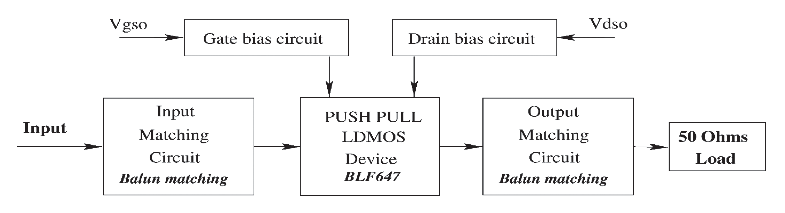
\includegraphics[width=3in]{Sample_Fig1.eps}\label{fig_first_case}}%
\hskip3pc
\subfloat[Case II]{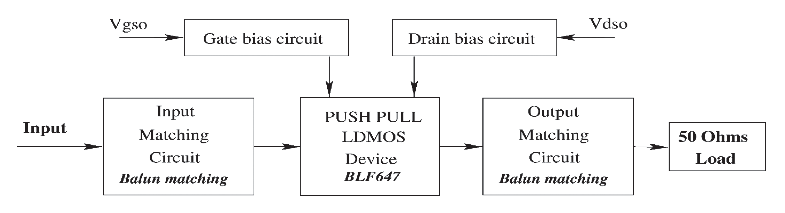
\includegraphics[width=3in]{Sample_Fig1.eps}\label{fig_second_case}}%
\caption[]{Sample sub figures in \LaTeX}
\label{fig_sim}
\end{figure*}
\end{verbatim}

\noindent The coding for a table is:

\begin{verbatim}
\begin{table}[!t]
\processtable{Insert table caption her\label{tab1}}
{\begin{tabular*}{\textwidth}{@{\extracolsep{\fill}}lllll@{}}
\hline
\TCH{Column head 1} & \TCH{Column head 2} & \TCH{Column head 3} &
\TCH{Column head 4} & \TCH{Column head 5}\\
\hline
Table body & Table body & Table body  & Table body  & Table body  \\
Table body & Table body & Table body  & Table body  & Table body  \\
Table body & Table body & Table body  & Table body  & Table body  \\
Table body & Table body & Table body  & Table body  & Table body  \\
Table body & Table body & Table body  & Table body  & Table body  \\
\end{tabular*}}{}
\end{table*}\end{verbatim}

As always with \LaTeX, the \verb|\label| must be after the
\verb|\caption|, and inside the figure or table environment. The reference for
figures and tables inside text can be made using the \verb|\ref{key}| command.


\section{Equations}\label{sec3.10}

Equations are used in the same way as described in the \LaTeX\ manual.
Equations are numbered consecutively, with equation numbers
in parentheses flush right.\noindent

\vskip1pc
\noindent For example, if you type
\begin{verbatim}
\begin{equation}\label{eq1}
\int^{r_2}_0 F(r,\varphi){\rm d}r\,{\rm d}\varphi = [\sigma r_2/(2\mu_0)]
\int^{\infty}_0\exp(-\lambda|z_j-z_i|)\lambda^{-1}J_1 (\lambda r_2)J_0
(\lambda r_i\,\lambda {\rm d}\lambda)
\end{equation}
\end{verbatim}
then you will get the following output:
\begin{equation}\label{eq1}
\int^{r_2}_0 F(r,\varphi){\rm d}r\,{\rm d}\varphi = [\sigma r_2/(2\mu_0)]\int^{\infty}_0
\exp(-\lambda|z_j-z_i|)\lambda^{-1}J_1 (\lambda r_2)J_0 (\lambda r_i\,\lambda {\rm d}\lambda)
\end{equation}
\AmS-\LaTeX{} has several environments that
make it easier to typeset complicated multiline displayed equations. These are explained in the
\AmS-\LaTeX{} User Guide. A \verb|subequation| environment is available to create equations with
sub-numbering of the equation counter. It takes one (optional)
argument to specify the way that the sub-counter should appear.


\section{Spanning equations}

In order to span the equations across two columns, please use the command
\verb+\begin{widetext}...\end{widetext}+ command as shown below:

\begin{verbatim}
\begin{widetext}
\begin{align} \label{d24} x_{\sigma+1} &= x_{\sigma} + \left( \dfrac{1-\alpha(t_\sigma)}
{M[\alpha(t_\sigma)]} + \dfrac{3h\alpha(t_\sigma)}{2M[\alpha(t_\sigma)]} \right)
\left\{-bx(t_\sigma-m_1) + a \sin [cx(t_\sigma-m_2)]\right\}  - \left( \dfrac{1-\alpha
(t_\sigma)}{M[\alpha(t_\sigma)]} + \dfrac{h \alpha(t_\sigma)}{2M[\alpha(t_\sigma)]}\right)
\nonumber\\ &\quad\times \left\{-bx(t_\sigma-m_1) + a \sin [cx(t_\sigma-m_2)]\right\}.
\end{align}
\end{widetext}
\end{verbatim}

Also include the package \verb+\usepackage{widetext-TI}+ in the preamble.

\section{Quotes and displayed text}
\label{sec3.11}

Quotes are indented from the left and right margins. There are various types of quotes:
short quote, long quote and display poetry.\vskip1pc

\noindent The coding for a short quote is \verb|\begin{quote}...\end{quote}|.
\begin{quote}
   This is a short quotation.  It consists of a
   single paragraph of text.  See how it is formatted.
\end{quote}

\noindent The coding for a long quote is \verb|\begin{quotation}...\end{quotation}|.

\begin{quotation}
   This is a longer quotation.  It consists of two
   paragraphs of text, neither of which are
   particularly interesting.

   This is the second paragraph of the quotation.  It
   is just as dull as the first paragraph.
\end{quotation}

\section{Listings}
\label{sec3.12}

Another frequently displayed structure is a list. There are various types of list:
numbered, itemized and bulleted. To create a bulleted list use the following:

\begin{verbatim}
\begin{itemize}
\item Bulleted list 1
\item Bulleted list 2
\item Bulleted list 3
\end{itemize}
\end{verbatim}

\noindent To create a numbered list use the following:

\begin{verbatim}
\begin{enumerate}
\item Numbered list 1
\item Numbered list 2
\item Numbered list 3
\end{enumerate}
\end{verbatim}

\noindent To create a description list use the following:

\begin{verbatim}
\begin{description}
\item Description list 1
\item Description list 2
\item Description list 3
\end{description}
\end{verbatim}

\section{Enunciations like theorem, lemma etc.}
\label{sec3.13}

The \AmS-\LaTeX\ package for enunciations (amsthm.sty) has been already loaded in the class file.

To get the theorem environment use the following:
\begin{verbatim}
\begin{theorem}
Theorem text. Theorem text. Theorem text.
Theorem text. Theorem text. Theorem text.
\end{theorem}
\end{verbatim}

and \verb|\newtheorem{theorem}{Theorem}| in the preamble.

Similarly, we can define for lemma, corollary, proposition, definition etc.

\section{Cross-referencing}
\label{sec3.14}

LATEX provides the following commands for cross referencing\vskip1pc

\noindent \verb|\label{marker}|, \verb|\ref{marker}| and \verb|\pageref{marker}|\vskip1pc

\noindent where marker is an identifier chosen by the user. LATEX replaces \verb|\ref| by
the number of the section, subsection, figure, table, or theorem after which
the corresponding \verb|\label| command was issued. \verb|\pageref| prints the page
number of the page where the \verb|\label| command occurred.

\section{Citations}

Citations are made with the \verb|\cite,\citep,\citet| command as usual. In this class file we have
used natbib.sty for cross references and reference style.

For bibliography the natbib package has been defined in the template as \verb|\usepackage[authoryear]{natbib}|
with \verb|\bibpunct[, ]{(}{)}{;}{a}{,}{;}| command

For more details about natbib.sty can be found at
http://ctan.org/tex-archive/macros/latex/contrib/natbib/

\section{Acknowledgements}

Acknowledgements and other unnumbered sections are created
using the \verb|\section*| command:

\begin{verbatim}
\section*{Acknowledgment}
\end{verbatim}

\section{Back Matter}

Please use the respective coding for back matter sections.

\begin{verbatim}

%%% For acknowledgment
\ack{Insert the Acknowledgment text here.}

%%% For Competing interests
\competing{Insert the Competing interests text here.}

%%% For contribution
\contribution{Insert the Contribution text here.}

%%% For funding
\funding{Insert the Funding interests text here.}

%%% For data availability
\data{Insert the Data availability text here.}

%%% For supplementary
\supplementary{Insert the supplementary text text here.}
\end{verbatim}


\section{References}
\label{sec3.18}

The reference entries can be \LaTeX\ typed bibliographies or generated through a BIB\TeX\ database.
BIB\TeX\ is an adjunct to \LaTeX\ that aids in the preparation of bibliographies. BIB\TeX\
allows authors to build up a database or collection of bibliography entries that may be used for many
manuscripts. They also save us the trouble of having to specify formatting. More details can be found
in the \textit{BIB\TeX\ Guide}. For \LaTeX\ reference entries use the
\verb|\begin{thebibliography}...\end{thebibliography}| environment (see below) to make references in your paper.
By default the class file will produce the unnumbered \LaTeX\ bibliography.

\begin{verbatim}
\begin{thebibliography}
\bibitem[Arendt et~al.(2016)]{bib1}
\textbf{Arendt, D., Musser, J. M., Baker, C. V., Bergman, A., Cepko, C., Erwin, D. H.,
Pavlicev, M., Schlosser, G., Widder, S., Laubichler, M. D. et al.} (2016). The
origin and evolution of cell types. \textit{Nat. Rev. Genet}. 17, 744--757.

\bibitem[Ben-Tabou et~al.(2010)]{bib2}
\textbf{Ben-Tabou de-Leon, S. B. and Davidson, E. H.} (2010). Information processing at
the foxa node of the sea urchin endomesoderm specification network. \textit{Proc. Natl
Acad. Sci}. USA 107, 10103--10108.

\bibitem[Calestani and Rogers (2010)]{bib3}
\textbf{Calestani, C. and Rogers, D. J.} (2010). Cis-regulatory analysis of the sea urchin
pigment cell gene polyketide synthase. \textit{Dev. Biol.} 340, 249--255.

\bibitem[Cameron and Davidson (1991)]{bib4}
\textbf{Cameron, R. A. and Davidson, E. H.} (1991). Cell type specification during sea
urchin development. \textit{Trends Genet.} 7, 212--218.


\bibitem[Cameron et~al.(1987)]{bib5}
\textbf{Cameron, R. A., Hough-Evans, B. R., Britten, R. J. and Davidson, E. H.} (1987).
Lineage and fate of each blastomere of the eight-cell sea urchin embryo. \textit{Genes
Dev.} 1, 75--85.

\bibitem[Croce and McClay (2010)]{bib6}
\textbf{Croce, J. C. and McClay, D. R.} (2010). Dynamics of Delta/Notch signaling on
endomesoderm segregation in the sea urchin embryo. \textit{Development} 137, 83--91.

\end{thebibliography}

\end{verbatim}

\section{Formatting}
\label{sec3.8}

Please use \LaTeX\ macros rather than the lower-level
\TeX\ macros such as \verb|\it|, \verb|\bf| and \verb|\tt|. The
\LaTeX\ macros offer much improved features. The following table summarizes the font
selection commands in \LaTeX.

\section*{\LaTeX\ text formatting commands}
\begin{tabular}{ll@{\hskip60pt}ll}
\verb|\textit|  & Italics      &\verb|\textsf|  & Sans Serif\\[3pt]
\verb|\textbf|  & Boldface     &\verb|\textsc|  & Small Caps\\[3pt]
\verb|\texttt|  & Typewriter   &\verb|\textmd|  & Medium Series\\[3pt]
\verb|\textrm|  & Roman        &\verb|\textnormal| & Normal Series\\[3pt]
\verb|\textsl|  & Slanted      &\verb|\textup|  & Upright Series
\end{tabular}


\section*{\LaTeX\ math formatting commands}
\begin{tabular}{ll@{\qquad}ll}
\verb|\mathit|     & Math Italics        &\verb|\mathfrak|   & Fraktur\\[3pt]
\verb|\mathbf|     & Math Boldface       &\verb|\mathbb|     & Blackboard Bold\\[3pt]
\verb|\mathtt|     & Math Typewriter     &\verb|\mathnormal| & Math Normal\\[3pt]
\verb|\mathsf|     & Math Sans Serif     &\verb|\boldsymbol| & Bold math for Greek letters\\[3pt]
\verb|\mathcal|    & Calligraphic        &                   & and other symbols
\end{tabular}

\section{Macro packages}
\label{sec4}

The commonly used packages which can be used frequently are:
\begin{verbatim}
amsmath         graphicx        rotating
amssymb         endnotes        subfigure
amsfonts        setspace        array
xspace          latexsym        url
amscd           multicol        algorithm
\end{verbatim}

If you wish to use other packages, these should be loaded
using the \verb|\usepackage| command in the preamble.

\appendix
\section{Appendix}
\label{sec3.16}

The \verb|\appendix| command signals that all subsequent sections are
appendices, and therefore the headings after \verb|\appendix| will be set
as appendix headings.

Note: All the figures, tables, equations, enunciations will be automatically
numbered as A.1, A.2, etc. in the appendix.


\end{document}
